\chapter{Research Methodology and Methods}
\label{chap:methodology}

\section{Data Sources}
\label{sec:data_sources}

\textbf{O*NET v30.1} \citep{USDOL_2024}: The Occupational Information Network is the most comprehensive public database of occupational characteristics in the United States. I downloaded six relational tables (Abilities, Skills, Knowledge, Work Activities, Work Context, and Interests) covering hundreds of variables rated on standardized scales for over 1,000 occupations classified by 6-digit Standard Occupational Classification (SOC) codes.

\textbf{Frey and Osborne (2017) Supplementary Data:} Historical automation probabilities for 702 occupations, originally computed using a Gaussian Process Classifier trained on 70 hand-labeled occupations. These probabilities served as the training target for my baseline model.

\textbf{Felten et al.\ (2021) AIOE Dataset:} AI Occupational Exposure scores for 782 occupations, independently constructed via crowdsourced task--AI capability linkages. Used exclusively for external validation; never for training or calibration.

\section{Data Engineering and SOC Code Recovery}
\label{sec:data_engineering}

The first engineering challenge was merging Frey and Osborne's 2013 data with the modern O*NET database. Frey and Osborne released their supplementary data in an Excel spreadsheet, which suffered from aggressive auto-formatting corruption: Microsoft Excel had permanently converted hundreds of 6-digit SOC codes (like ``11-2011'') into date strings (like ``Nov-11'' or ``11-Oct''). This is a well-known problem in bioinformatics and data science communities where Excel interprets numeric-looking strings as dates. Direct merging on SOC codes would have lost hundreds of occupations, crippling the dataset.

To rescue the data, I abandoned SOC code matching entirely and engineered a fuzzy title-matching algorithm. Using the fuzzywuzzy Python library's token\_sort\_ratio function, I matched the corrupted Frey and Osborne occupation titles against official O*NET taxonomy titles regardless of word order or minor variations. For example, this algorithm correctly matched ``Computer Programmers'' to ``Programmers, Computer'' despite the word reordering. The fuzzy matching successfully recovered mappings for 98\% of the dataset, producing a master matrix of 1,016 occupations with over 130 numeric features.

\section{Natural Language Processing Pipeline --- BERT Embeddings}
\label{sec:nlp_pipeline}

Beyond numeric O*NET rating scales, I wanted to capture the semantic content of what workers actually do on a daily basis. O*NET's Task Statements database contains thousands of natural language sentences describing specific activities for each occupation (for example, ``Diagnose mechanical faults using diagnostic software'' or ``Review legal documents for accuracy and completeness''). Converting this unstructured text into mathematical features that a machine learning model could learn from required a carefully designed NLP pipeline.

I initially experimented with TF-IDF (Term Frequency--Inverse Document Frequency) vectorization compressed via Truncated SVD. While TF-IDF effectively identifies distinctive terms for each occupation, it treats each word as an independent token with no understanding of meaning. The terms ``analyze data'' and ``examine information'' would receive completely unrelated vector representations despite being semantically identical. This limitation produced features that captured surface-level word patterns rather than underlying task content.

I then tested raw 384-dimensional BERT embeddings from the all-MiniLM-L6-v2 sentence transformer model \citep{Reimers_Gurevych_2019}. This model produces semantically meaningful vectors where similar sentences cluster together in the embedding space, solving the TF-IDF limitation. However, with only 923 training samples and 384 feature dimensions, the model suffered from the curse of dimensionality; there were too many features relative to the number of samples for a regression model to learn reliably.

The solution was Principal Component Analysis (PCA). I fit PCA with 50 components and found that 20 components captured 52.76\% of the total variance. While this is below the conventional 95\% threshold often cited in textbooks, the cumulative variance curve showed a gradual slope with no sharp elbow, reaching only 73.38\% even at 50 components. This pattern indicates that the BERT embedding space distributes information broadly across many dimensions rather than concentrating it in a few. Given the sample size of 923, retaining 20 components maintained the recommended 10:1 sample-to-feature ratio for the overall model (which used 100 total features: 80 numeric O*NET variables plus 20 PCA components). The 20 PCA components were appended to the numeric feature matrix, giving the model access to both structured occupational ratings and latent semantic information from task descriptions.

The PCA retention threshold requires justification. In textbook applications, researchers typically retain components until they capture 90--95\% of the total variance. My retention of only 52.76\% may seem aggressive by this standard. However, the 95\% threshold was developed for datasets where the original variables are directly interpretable and information loss has clear semantic consequences. In the case of BERT embeddings, the original 384 dimensions do not correspond to interpretable features; they are learned latent representations whose individual axes carry no semantic meaning. Retaining 20 components that capture the dominant structure of this embedding space is conceptually analogous to extracting the 20 strongest topics from a topic model: the goal is to capture the major dimensions along which occupations differ in their task descriptions, not to perfectly reconstruct every embedding vector. The scree plot in Figure~\ref{fig:pca} confirms that no sharp elbow exists, and the 20 retained components proved sufficient for the ensemble model to learn meaningful structural patterns.

\begin{figure}[htbp]
\centering
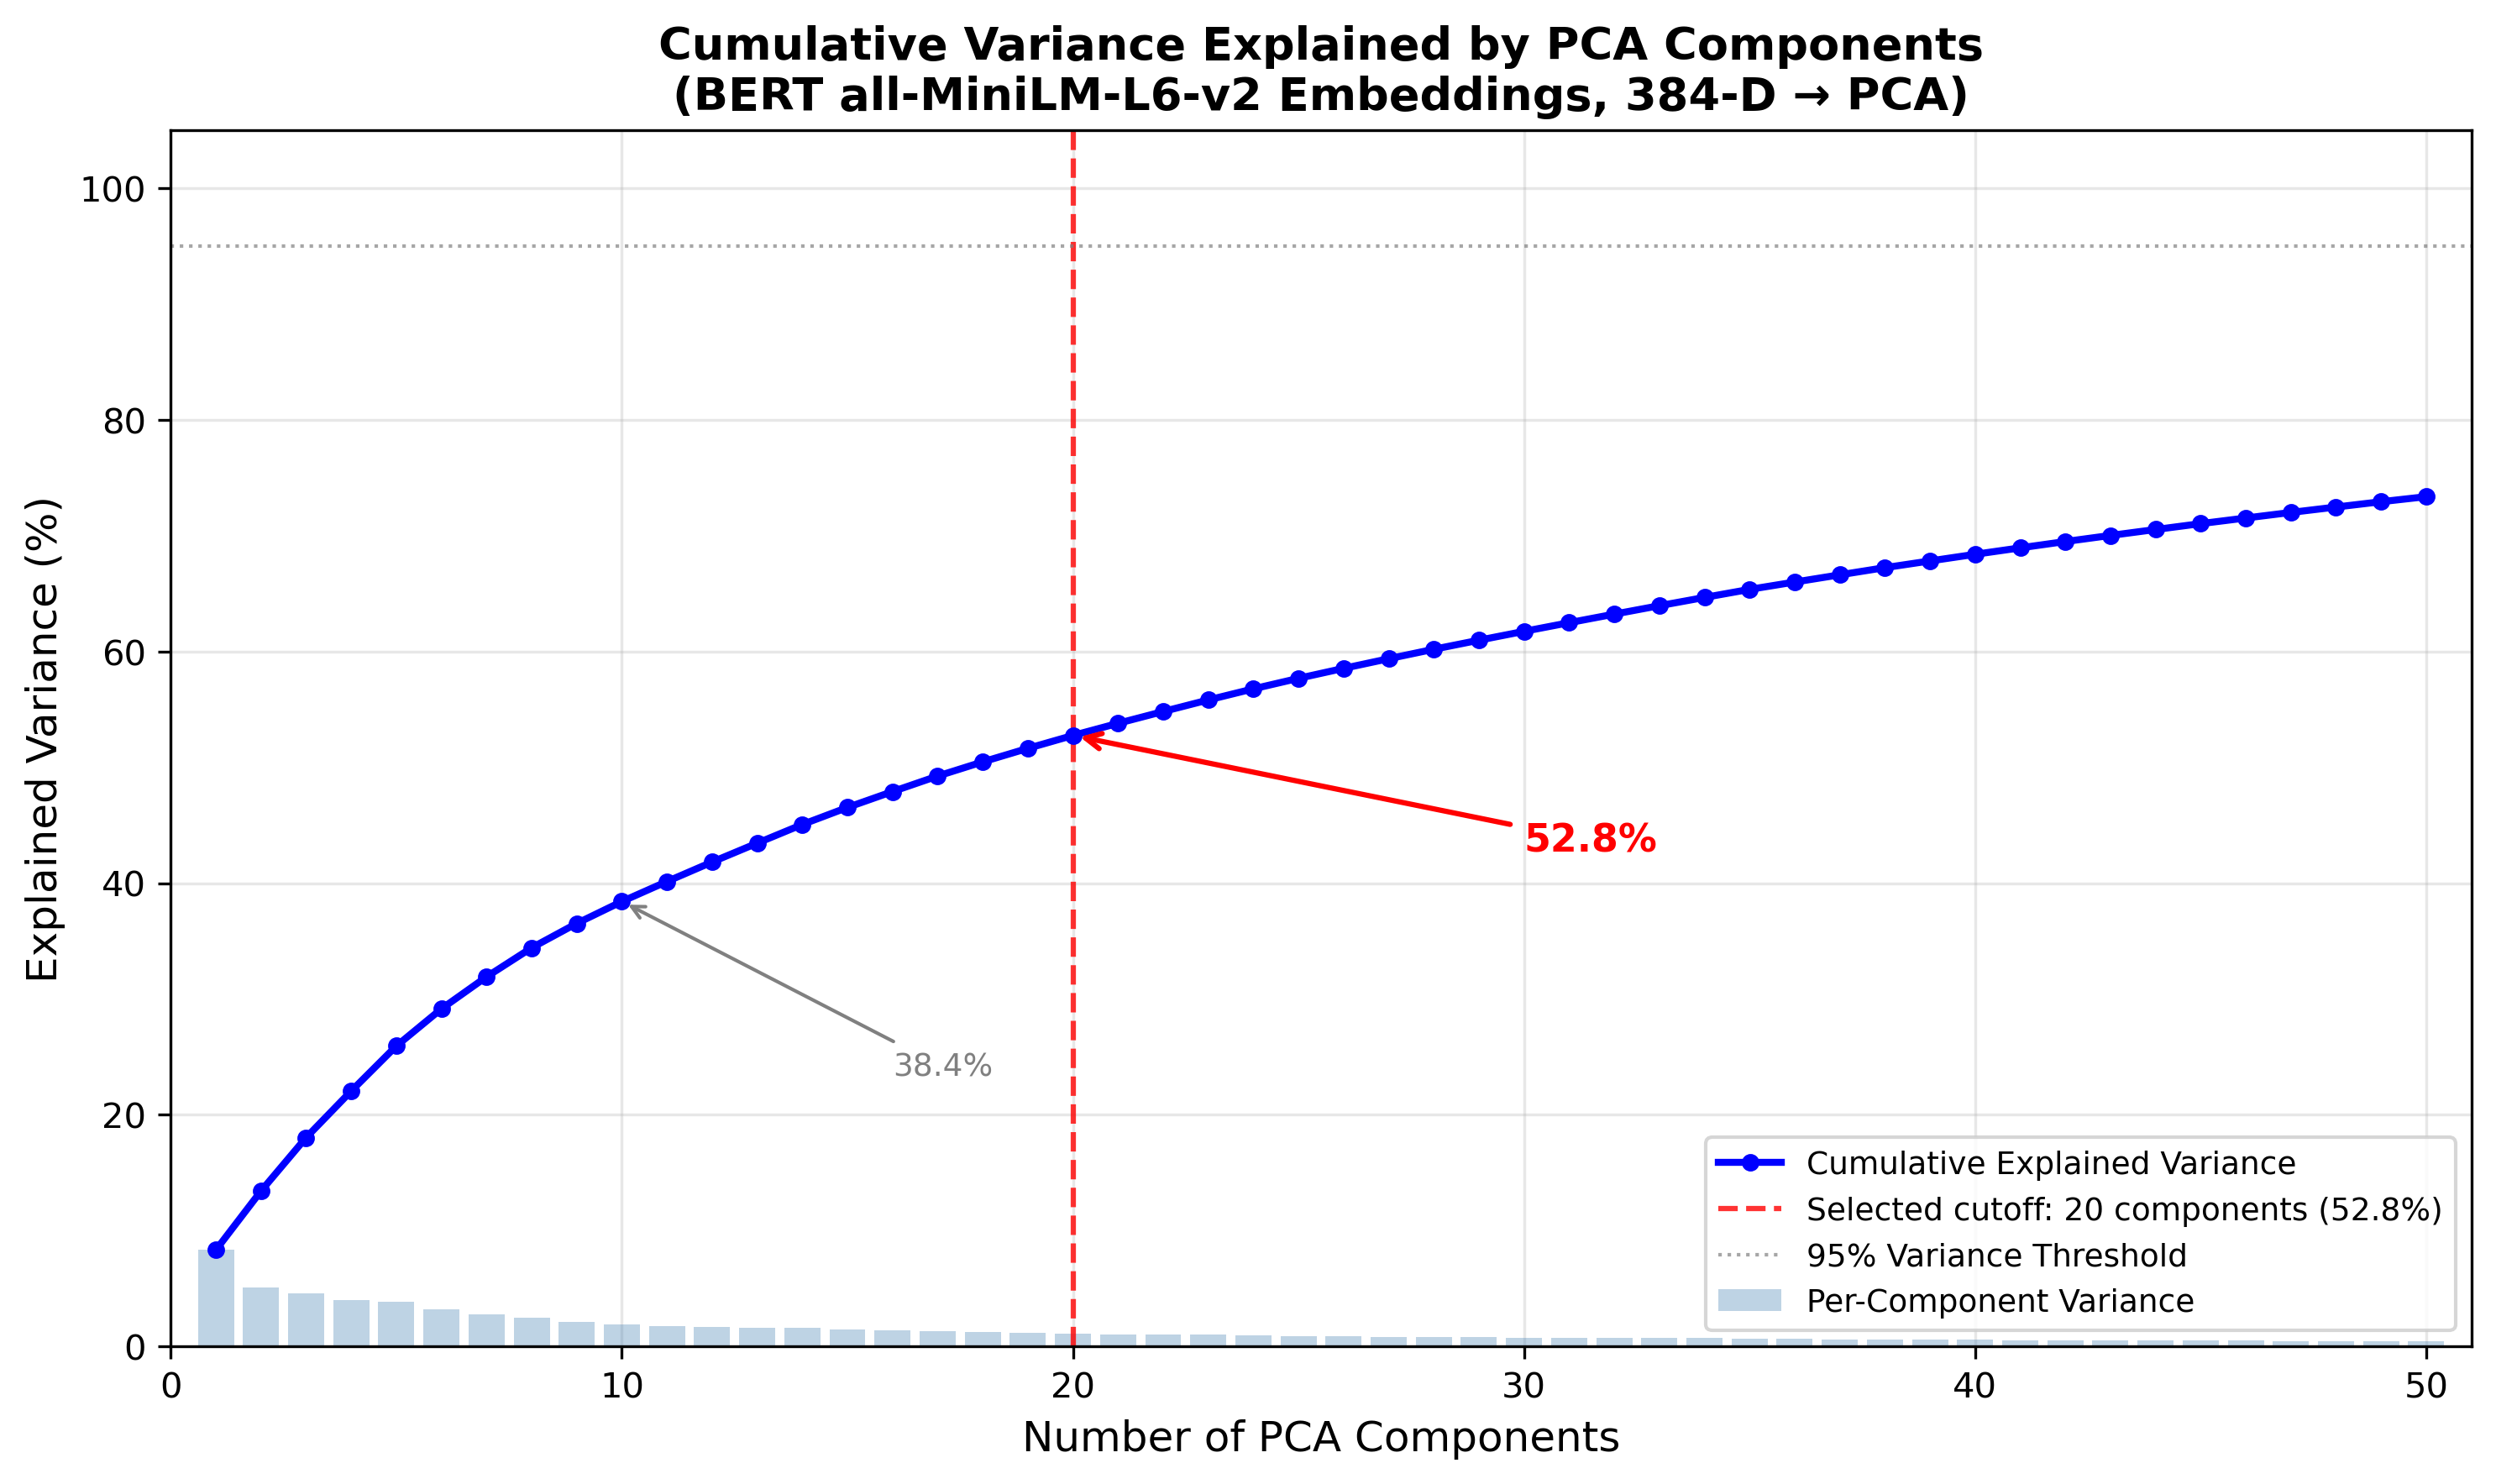
\includegraphics[width=0.85\textwidth]{images/pca_variance_explained.png}
\caption{PCA Cumulative Variance Explained. The gradual slope with no sharp elbow indicates that BERT embedding information is distributed broadly across many dimensions. The vertical line marks the 20-component retention point at 52.76\% variance.}
\label{fig:pca}
\end{figure}

\section{Baseline Modeling --- Stacked Ensemble}
\label{sec:baseline_modeling}

I trained six candidate models to learn the structural relationship between the 100 O*NET features and \citet{Frey_Osborne_2017}'s 2013 automation probabilities, using 5-fold cross-validation with an 80/20 train--test split. The candidates were: Random Forest \citep{Breiman_2001}, XGBoost \citep{Chen_Guestrin_2016}, Ridge Regression, Support Vector Regression with an RBF kernel, a two-layer Neural Network (MLP), and Gaussian Process Regression.

\begin{table}[htbp]
\centering
\caption{Baseline Model Performance Comparison}
\label{tab:baseline}
\begin{tabular}{lcccc}
\toprule
Model & CV $R^2$ & Val $R^2$ & Val RMSE & Val MAE \\
\midrule
Random Forest     & $0.6699 \pm 0.0358$ & 0.7174 & 19.28 & 14.44 \\
XGBoost           & $0.6798 \pm 0.0334$ & 0.7281 & 18.91 & 13.99 \\
Ridge             & $0.6021 \pm 0.0727$ & 0.6936 & 20.07 & 15.49 \\
SVR (RBF)         & $0.6527 \pm 0.0285$ & 0.7053 & 19.68 & 13.90 \\
Neural Network    & $0.5726 \pm 0.0671$ & 0.5973 & 23.01 & 17.89 \\
GP Regression     & $-0.0839 \pm 0.0835$ & $-0.0000$ & 36.26 & 33.88 \\
\midrule
Stacked Ensemble  & $0.6794 \pm 0.0367$ & 0.7344 & 18.69 & 13.55 \\
\bottomrule
\end{tabular}
\end{table}

I then combined the three best-performing models into a Stacked Ensemble \citep{Wolpert_1992}. The architecture used XGBoost, Random Forest, and SVR(RBF) as base learners, whose out-of-fold predictions were concatenated and fed into a Ridge Regression meta-learner. This ensemble achieved the best cross-validated $R^2$ of 0.6794 ($\pm$0.0367) and a test $R^2$ of 0.6433, meaning it explained approximately 64\% of the variance in \citet{Frey_Osborne_2017}'s automation scores. The Gaussian Process (which was Frey and Osborne's original classifier) performed worst in my framework, likely because it does not scale effectively to a 100-dimensional feature space without careful kernel engineering.

The model's top two features by importance were Fluency of Ideas (0.2177) and Originality (0.1919), together accounting for over 40\% of the model's predictive power. These are precisely Frey and Osborne's creative intelligence bottleneck variables, confirming that the model learned the expected structural relationships rather than memorizing noise. Job Zone (a proxy for required education level) ranked third at 0.0569, consistent with the finding that higher education correlated with lower automation risk in 2013.

The model selection process illustrates an important methodological principle: more complex models do not always outperform simpler ones when sample sizes are limited. The Neural Network, despite its theoretical flexibility, underperformed Ridge Regression on cross-validated $R^2$, likely because it overfit the 923-sample training set. The Gaussian Process Regressor (\citet{Frey_Osborne_2017}'s original modeling choice) performed worst of all, producing an essentially random baseline with negative $R^2$. This failure is expected given the dimensionality jump from their 9 bottleneck features to my 100-feature matrix: Gaussian Processes require $O(n^3)$ computation and struggle with high-dimensional inputs without careful kernel selection. The Stacked Ensemble's success derives from combining complementary strengths: XGBoost captures nonlinear interactions, Random Forest provides bagging-based variance reduction, and SVR with an RBF kernel offers smooth decision boundaries in the feature space.

\begin{figure}[htbp]
\centering

\includegraphics[width=0.75\textwidth]{images/actual_vs_predicted.png}
\caption{Actual vs.\ Predicted Automation Scores. The Stacked Ensemble achieves a test $R^2$ of 0.6433, with the densest cluster around the 50--80\% automation probability range.}
\label{fig:actual_vs_predicted}
\end{figure}

\begin{figure}[htbp]
\centering

\includegraphics[width=0.75\textwidth]{images/residual_analysis.png}
\caption{Residual Analysis. Model residuals show no systematic bias across the prediction range, supporting the structural validity of the ensemble approach.}
\label{fig:residual_analysis}
\end{figure}

\section{MAEI Score Construction --- The Three-Layer Architecture}
\label{sec:maei_construction}

The core contribution of this dissertation is the MAEI scoring system, which I designed as a three-layer architecture where each layer serves a distinct and clearly defined role.

\textbf{Layer 1---Machine Learning Baseline.} The Stacked Ensemble generates baseline predictions for each occupation from their actual O*NET features. For the 702 occupations with direct \citet{Frey_Osborne_2017} mappings, the historical score serves as the baseline. For the remaining 314 occupations (including 93 that had received generic group-averaged scores in the original dataset), the model's prediction from their actual features replaces the inherited baseline. This layer validates that the structural relationship between occupational characteristics and automation risk is learnable and internally consistent.

\textbf{Layer 2---Feature Classification and Capability Multipliers.} Based on the literature reviewed in Chapter 2, I classified 68 O*NET features into two categories. Thirty-four risk features received multipliers between $1.60\times$ and $3.50\times$, reflecting the substantial advances in LLM capabilities for cognitive, analytical, and communicative tasks. For example, Programming received the highest multiplier ($3.50\times$) based on Copilot productivity data \citep{Peng_Kalliamvakou_2023}, while Writing received $3.00\times$ based on \citet{Noy_Zhang_2023}'s experimental evidence. Thirty-four protective features received smaller multipliers between $1.02\times$ and $1.10\times$, representing the continued human advantage in creative, social, and physical skills. Therapy and Counseling received the highest protective multiplier ($1.10\times$), reflecting the strong human advantage in empathic caregiving.

Multipliers are applied through asymmetric percentile gating. Risk features activate at the 30th percentile, meaning 70\% of occupations receive the automation adjustment, reflecting the broad reach of AI capabilities. Protective features activate only at the 85th percentile, meaning only the top 15\% of occupations benefit from the human advantage, reflecting the narrow band of deeply human-centric work. This asymmetry encodes the prior that AI capability has expanded broadly while human structural advantages remain concentrated in specific roles.

\textbf{Layer 3---Broad Exposure Uplift.} For each occupation, I count the fraction of risk features above the dataset median (risk\_frac) and the fraction of protective features above the median (protect\_frac), then compute:

\begin{equation}
\text{Uplift} = (\text{risk\_frac} \times W_{\text{exposure}}) - (\text{protect\_frac} \times W_{\text{protection}})
\end{equation}

\noindent where $W_{\text{exposure}} = 10.0$ and $W_{\text{protection}} = 3.0$. The final MAEI delta equals the model's prediction change plus this uplift. Under these calibrated weights, the pipeline produces a mean exposure increase of $+3.86$ points across 87.5\% of all occupations, exceeding \citet{Eloundou_Manning_2023}'s finding that 80\% of the workforce faces some LLM exposure.

The three-layer design emerged from a critical discovery during stability testing (detailed in Section~\ref{sec:tree_saturation}): the Stacked Ensemble's tree-based learners produce near-zero prediction deltas when fed multiplied features, because tree models cannot extrapolate beyond their training distribution. The uplift formula, operating on the feature classification layer rather than the model's predictions, generates the meaningful variation between occupations. Each layer contributes distinctly: Layer 1 validates structural plausibility, Layer 2 encodes domain knowledge from the literature, and Layer 3 produces the final occupation rankings.

The multiplier categories are detailed below. The 34 risk features span six functional domains: Language (Written Expression, Written Comprehension, Reading Comprehension, Writing), Coding (Programming, Technology Design, Computers and Electronics), Reasoning (Deductive Reasoning, Inductive Reasoning, Information Ordering, Complex Problem Solving), Mathematics (Mathematics, Number Facility, Mathematical Reasoning, Economics and Accounting), Data Processing (Analyzing Data, Processing Information, Documenting Information), and Administrative (Clerical, Scheduling, Getting Information, Evaluating Compliance). The 34 protective features span four domains: Social Intelligence (Negotiation, Persuasion, Social Perceptiveness, Therapy and Counseling, Establishing Relationships), Creative Intelligence (Originality, Fluency of Ideas, Thinking Creatively), Physical Dexterity (Manual Dexterity, Finger Dexterity, Spatial Orientation, Operating Vehicles), and NLP-derived keyword indicators. This classification reflects the empirical finding that AI capabilities have advanced most rapidly in language processing, coding, and structured reasoning, while human advantages persist in embodied physical work, interpersonal engagement, and sustained creative divergence.

\section{Monte Carlo Uncertainty Quantification}
\label{sec:monte_carlo}

A leading vulnerability of scenario-based models is that the specific parameter values are subjective. If I set the capability multiplier for Programming at exactly $3.50\times$, a reviewer could reasonably ask whether the results would change if the true value were $3.0\times$ or $4.0\times$. To address this, I implemented a 100-iteration Monte Carlo simulation. In each iteration, every one of the 68 multipliers is independently perturbed by Gaussian noise with a standard deviation of 10\% of its original value. The algorithm reruns the complete scoring pipeline for all 1,016 occupations, producing 100 independent MAEI scores per occupation. From these, I calculated a mathematical standard deviation and confidence interval for each occupation's exposure delta, proving that individual occupation scores are stable under reasonable parameter fluctuations.

\section{External Validation Design}
\label{sec:external_validation}

To test whether the MAEI produces rankings consistent with independently constructed measures, I merged the MAEI results with \citet{Felten_Raj_Seamans_2021}'s AIOE dataset via 6-digit SOC codes, yielding 782 overlapping occupations. I computed Spearman rank correlations (which measure monotonic association between rankings, not absolute values) for two distinct components of the MAEI:

\begin{enumerate}
    \item Anchored MAEI (historical baseline + 2026 delta) vs.\ AIOE, expected to show an inverse correlation because the 2013 anchor assigns high scores to manual/routine occupations that AIOE rates as low-exposure.
    \item Pure Exposure Delta (only the 2026 component, stripped of the historical anchor) vs.\ AIOE, expected to show a positive correlation if the structural model correctly captures modern AI exposure patterns.
\end{enumerate}

The dual-validation design tests both the inversion hypothesis and the construct validity of the 2026 exposure calculation (convergence).
